\documentclass[twoside,11pt,openright]{report}
%DIF LATEXDIFF DIFFERENCE FILE
%DIF DEL ./../afleveret/270315/thesis.tex   Thu Apr 16 14:25:17 2015
%DIF ADD thesis.tex                         Sat Apr 18 16:36:37 2015

\usepackage[utf8]{inputenc}
\usepackage[american]{babel}
\usepackage{a4}
\usepackage{latexsym}
\usepackage[numbers]{natbib}
%\usepackage[square,semicolon,sort,longnamesfirst]{natbib}
\usepackage{amssymb}
\usepackage{amsmath}
\usepackage{epsfig}
\usepackage{graphicx}
\usepackage[T1]{fontenc}
\usepackage{lmodern}
\usepackage{color}
\usepackage{datetime}
\usepackage{epstopdf} 

\renewcommand*\ttdefault{txtt}

\newcommand{\todo}[1]{{\color[rgb]{.5,0,0}\textbf{$\blacktriangleright$#1$\blacktriangleleft$}}}

\newtheorem{innercustomlem}{Lemma}
\newenvironment{customlem}[1]
  {\renewcommand\theinnercustomlem{#1}\innercustomlem}
  {\endinnercustomlem}

\newtheorem{innercustomthm}{Theorem}
\newenvironment{customthm}[1]
  {\renewcommand\theinnercustomthm{#1}\innercustomthm}
  {\endinnercustomthm}



% see http://imf.au.dk/system/latex/bog/
%DIF PREAMBLE EXTENSION ADDED BY LATEXDIFF
%DIF UNDERLINE PREAMBLE %DIF PREAMBLE
\RequirePackage[normalem]{ulem} %DIF PREAMBLE
\RequirePackage{color}\definecolor{RED}{rgb}{1,0,0}\definecolor{BLUE}{rgb}{0,0,1} %DIF PREAMBLE
\providecommand{\DIFadd}[1]{{\protect\color{blue}\uwave{#1}}} %DIF PREAMBLE
\providecommand{\DIFdel}[1]{{\protect\color{red}\sout{#1}}}                      %DIF PREAMBLE
%DIF SAFE PREAMBLE %DIF PREAMBLE
\providecommand{\DIFaddbegin}{} %DIF PREAMBLE
\providecommand{\DIFaddend}{} %DIF PREAMBLE
\providecommand{\DIFdelbegin}{} %DIF PREAMBLE
\providecommand{\DIFdelend}{} %DIF PREAMBLE
%DIF FLOATSAFE PREAMBLE %DIF PREAMBLE
\providecommand{\DIFaddFL}[1]{\DIFadd{#1}} %DIF PREAMBLE
\providecommand{\DIFdelFL}[1]{\DIFdel{#1}} %DIF PREAMBLE
\providecommand{\DIFaddbeginFL}{} %DIF PREAMBLE
\providecommand{\DIFaddendFL}{} %DIF PREAMBLE
\providecommand{\DIFdelbeginFL}{} %DIF PREAMBLE
\providecommand{\DIFdelendFL}{} %DIF PREAMBLE
%DIF END PREAMBLE EXTENSION ADDED BY LATEXDIFF

\begin{document}

%%%%%%%%%%%%%%%%%%%%%%%%%%%%%%%%%%%%%%%%%%%%%%%%%%%%%%%%%%%%%%%%%%%%%%%

\pagestyle{empty} 
\pagenumbering{roman} 
\vspace*{\fill}\noindent{\rule{\linewidth}{1mm}\\[4ex]
{\Huge\sf 2D Orthogonal Range Search}\\[2ex]
{\huge\sf Mads Ravn, 20071580}\\[2ex]
\noindent\rule{\linewidth}{1mm}\\[4ex]
\noindent{\Large\sf Master's Thesis, Computer Science\\[1ex] 
\monthname\ \the\year  \\[1ex] Advisor: Kasper Green Larsen\\[15ex]}\\[\fill]}
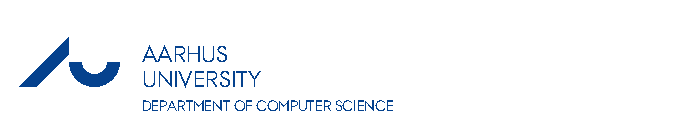
\epsfig{file=logo.eps}\clearpage

%%%%%%%%%%%%%%%%%%%%%%%%%%%%%%%%%%%%%%%%%%%%%%%%%%%%%%%%%%%%%%%%%%%%%%%

\pagestyle{plain}
\chapter*{Abstract}
\addcontentsline{toc}{chapter}{Abstract}

\todo{in English\dots}

\chapter*{Resum\'e}
\addcontentsline{toc}{chapter}{Resum\'e}

\todo{in Danish\dots}

\chapter*{Acknowledgements}
\addcontentsline{toc}{chapter}{Acknowledgments}

\todo{\dots}

\vspace{2ex}
\begin{flushright}
  \emph{Mads Ravn,}\\
  \emph{Aarhus, \today.}
\end{flushright}

\tableofcontents
\pagenumbering{arabic}
\setcounter{secnumdepth}{2}

%%%%%%%%%%%%%%%%%%%%%%%%%%%%%%%%%%%%%%%%%%%%%%%%%%%%%%%%%%%%%%%%%%%%%%%


\chapter{Introduction}
\label{ch:intro}

\noindent \emph{Orthogonal range searching} is one of the most fundamental and well-studied problems in computational geometry. Even with extensive research over three decades a lot of questions remain. In this thesis we will focus on $2D$ orthogonal range searching: Given $n$ points from $\mathbb{R}^2$ we want to insert them into a data structure which will be able to efficiently report which \DIFdelbegin \DIFdel{$k$ }\DIFdelend points lie within a given axis-aligned query rectangle $\mathbb{Q} \subseteq \mathbb{R}^2$.
\DIFdelbegin \DIFdel{This querycan be defined as two corners of a rectangle, the lower left corner and the upper right corner, seeing as the query range is orthogonal to the axes.}\DIFdelend 

\DIFaddbegin \begin{figure}[h]
    \centering
    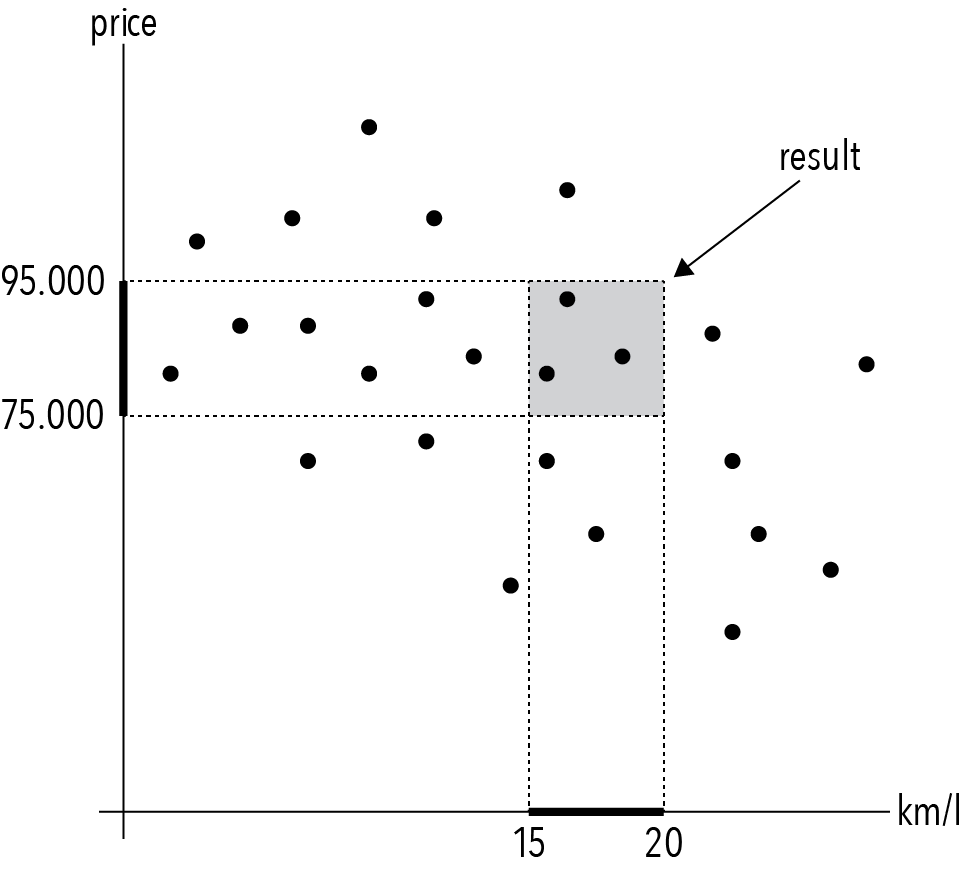
\includegraphics[width = 0.85\textwidth]{pictures/introduction.png}
    \caption{\DIFaddFL{Example of an orthogonal range query}}\label{fig:example}
\end{figure}

\noindent \DIFadd{Consider a database of vehicles for sale. Each vehicle has measurable}\todo{andet ord} \DIFadd{properties like price, the year the model was released, engine size, amount of doors, gasoline consumption in kilometers per liter, size  and maximum speed. With a $2$-dimensional query, two properties can be picked and a range for both properties can be set. A point in the graph reprensent the ID of the car with which the car can be looked up in the database to find the other properties of the car. Given the ranges on two properties we want to find those of the cars in the database which lie within the search query. Figure~\ref{fig:example} shows an example of such a search query. A buyer is interested in finding cars which cost between $75,000$ and $95,000$ and can drive between $15$ and $20$ kilometers per liter of gasolin. The points within the gray area represent cars which fit these criteria.}\\

\DIFaddend The objective of this thesis is to study a variety of \emph{orthogonal range searching} data structures. The main focus will be to introduce the \emph{Simple Range Search} data structure. It is a simplification of an orthogonal range searching data structure by \citet{chanetal}, which will be referred to as the \emph{Original Range Search} data structure. We are going to describe the kd-tree which will be the \DIFdelbegin \DIFdel{baseline }%DIFDELCMD < \todo{andet ord} %%%
\DIFdel{in our comparison }\DIFdelend \DIFaddbegin \DIFadd{reference data structure in our analysis }\DIFaddend of the Simple Range Search data structure. We are going to describe the range tree which shares some of properties of the Simple Range Search and Original Range Search data structures.

We show that a range query to the Simple Range Search data structure has a faster worst-case running time than a range query to the kd-tree. We also \DIFdelbegin \DIFdel{wish to }\DIFdelend show that the Simple Range Search data structure is able to compete with the kd-tree, and even outperform the kd-tree in some cases. \todo{Mere ...} \DIFaddbegin \\ 
\DIFaddend 


The model of computation used in this thesis is the \DIFaddbegin \DIFadd{$w$-bit }\DIFaddend word-RAM model \DIFdelbegin \DIFdel{as described by \mbox{%DIFAUXCMD
\citet{wordram}
}%DIFAUXCMD
}\DIFdelend \DIFaddbegin \DIFadd{by \mbox{%DIFAUXCMD
\citet{fredman}
}%DIFAUXCMD
}\DIFaddend . In the word-RAM model of computation, the memory is divided into words of $w$ bits. Given an \DIFdelbegin \DIFdel{input $I[1..n]$ with elements }\DIFdelend \DIFaddbegin \DIFadd{array $A[1..n]$ containing $n$ points with coordinates }\DIFaddend from a universe $U$, a word will have enough bits to store the integer address of any index into \DIFdelbegin \DIFdel{$I$ }\DIFdelend \DIFaddbegin \DIFadd{$A$ }\DIFaddend and enough bits to store any element from $U$. Thus, $w = \Omega(\lg n)$ and $w = \Omega(\lg U)$. Under the word-RAM model all standard word operations take constant time. This includes standard word operation from modern programming languages such as integer addition, subtraction, multiplication, division, shifts and the bit-wise operators AND, OR and XOR. Reading a single word from memory or writing a single word to memory also takes constant time. The number of bits in a word is found by the largest element which has to fit into a word. This means that it is often possible to divide the word into smaller logical blocks which can fit more than one integer. \todo{Indivisibility af pointer machine relevant?} \\


\noindent \textbf{Outline.} Has yet to be written. \\

\noindent \textbf{Notation.} The set of integers $\{i, i+1, \dots, j-1, j\}$ is denoted by $[i,j]$. When no base is explicitely given logarithm will have base $2$. $\epsilon$ is an arbitrary small constant greater than $0$. Given an array $A$, $A[i]$ denotes the entry with index $i$ in $A$ and $A[i,j]$ denotes the subarray containing the entries from $i$ to $j$ in $A$\DIFaddbegin \DIFadd{, including both $A[i]$ and $A[j]$}\DIFaddend . $A[1..n]$ denotes an array $A$ of size $n$ with entries $1$ to $n$. Throughout the thesis the successor of $x$ in a set will be meant as the \DIFdelbegin \DIFdel{first }\DIFdelend \DIFaddbegin \DIFadd{smallest }\DIFaddend number which is greater or equal to $x$ in that set - \DIFaddbegin \DIFadd{symmetrically, }\DIFaddend the same applies for predecessor of $x$ \DIFaddbegin \DIFadd{which is the biggest number less or equal to $x$}\DIFaddend . The work will be done under the assumption that no two points will  have the same x-coordinate and no two points will have the same y-coordinate. This is a unrealistic assumption in practice, but it can easily be remedied by having the points lie in a \DIFdelbegin \DIFdel{composite-number space }\DIFdelend \DIFaddbegin \emph{\DIFadd{composite-number space}} \DIFaddend since we only need a total ordering of our points.





%%%%%%%%%%%%%%%%%%%%%%%%%%%%%%%%%%%%%%%%%%%%%%%%%%%%%%%%%%%%%%%%%%%%%%%
\part{Theory}

\chapter{Related Work}
\label{ch:relatedwork}

This chapter will describe two well-known data structures for static range searching: the kd-tree and the range tree. The kd-tree is the current de facto standard for static range searching because of its low space complexity. It has a space complexity of $\mathcal{O}(n)$ and a running time of $\mathcal{O}(\sqrt{n} + k)$ where $k$ is the number of results reported. In practise it uses the exact same amount of words as it holds elements\DIFaddbegin \DIFadd{\mbox{%DIFAUXCMD
\cite{compgeo}
}%DIFAUXCMD
}\DIFaddend . The range tree uses $\mathcal{O}(n \lg n)$ words of space and has a running time of $\mathcal{O}(\lg^2 n + k)$ without \emph{fractional cascading} and a running time of $\mathcal{O}(\lg n + k)$ with fractional cascading. The difference between the space complexities of the kd-tree and the range tree is a factor $\mathcal{O}(\lg n)$ which can become an issue when dealing with very large datasets and a limited amount of main memory. This factor can grow big for large datasets and is the reason why kd-trees are prefered in practise.

The kd-tree will be used as a \DIFdelbegin \DIFdel{baseline }%DIFDELCMD < \todo{andet ord} %%%
\DIFdelend \DIFaddbegin \DIFadd{reference in the }\DIFaddend comparison against the Simple Range Search data structure since they have the same space complexity. This property makes the Simple Range Search data structure quite attractive. The range tree will be used to show how much the running time can be decreased by increasing the space complexity by a factor of $\mathcal{O}(\lg n)$. The range tree will also be used to introduce some of the ideas behind the Simple Range Search and Original Range Search data structures, which is where \citet{chanetal} drew some of their inspiration.

The query time of the main data structures in this chapter are all \emph{output-sensitive}, meaning that their running time depends on the amount of results found. The data structures themselves are static: After the initial construction of the data structures they will not be altered by insertions or deletions. \todo{more} 

\section{kd-trees}
\label{sect:kdtrees}

The current standard of range reporting using linear space is the kd-tree. This data structure will be used as a reference point when evaluting the results of the primary work of the thesis. With linear space it is a fitting data structure for range reporting on the RAM, and a practical solution. \DIFaddbegin \DIFadd{The kd-tree with $n$ points can be represented as an array $A[1..n]$.}\todo{Beskriver det fint nok at størrelsen er $n$?}
\DIFaddend 

\DIFaddbegin \begin{figure}[h]
    \centering
    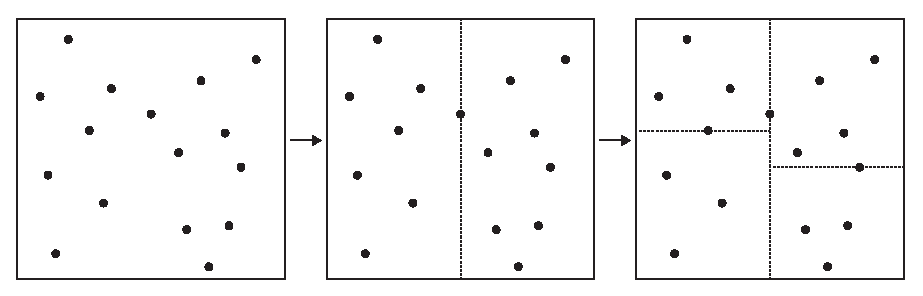
\includegraphics[width = 1.0\textwidth]{pictures/kd_subdivision.eps}
    \caption{\DIFaddFL{Showing the subdivision of points in a node: First dividing the points by the x-median, and then by the y-median}}\label{fig:kdsubdivision}
\end{figure}


\DIFaddend A kd-tree is constructed recursively: Given $n$ points, the median of the points with respect to x is found. All points which has an x-coordinate larger than the median goes to the right child, while points which has an x-coordinate smaller than the median, and the median point, goes to the left child. At the next level the points \DIFaddbegin \DIFadd{of each node }\DIFaddend will be divided in a similar fashion, this time using the y-median and the y-coordinates instead. \DIFaddbegin \DIFadd{This is shown on figure~\ref{fig:kdsubdivision}. }\DIFaddend When dividing $n$ points, the median will be chosen as the $\lceil n/2 \rceil$-th smallest number\DIFdelbegin \DIFdel{\mbox{%DIFAUXCMD
\cite{compgeo}
}%DIFAUXCMD
}\DIFdelend . Therefore a node will contain the line dividing the points given to its left child from the points given to its right child.
Alternating between focussing on the x-coordinates or the y-coordinates at each level, the points are divided until only one point remains in a node. This node will then be a leaf containing that point. Thus, we end up with $n$ leaves. This data structure \DIFdelbegin \DIFdel{takes up }\DIFdelend \DIFaddbegin \DIFadd{uses }\DIFaddend $\mathcal{O}(n)$ \DIFdelbegin \DIFdel{space.
}\DIFdelend \DIFaddbegin \DIFadd{words of space. }\\
\DIFaddend 

\DIFaddbegin \begin{figure}[h]
    \centering
    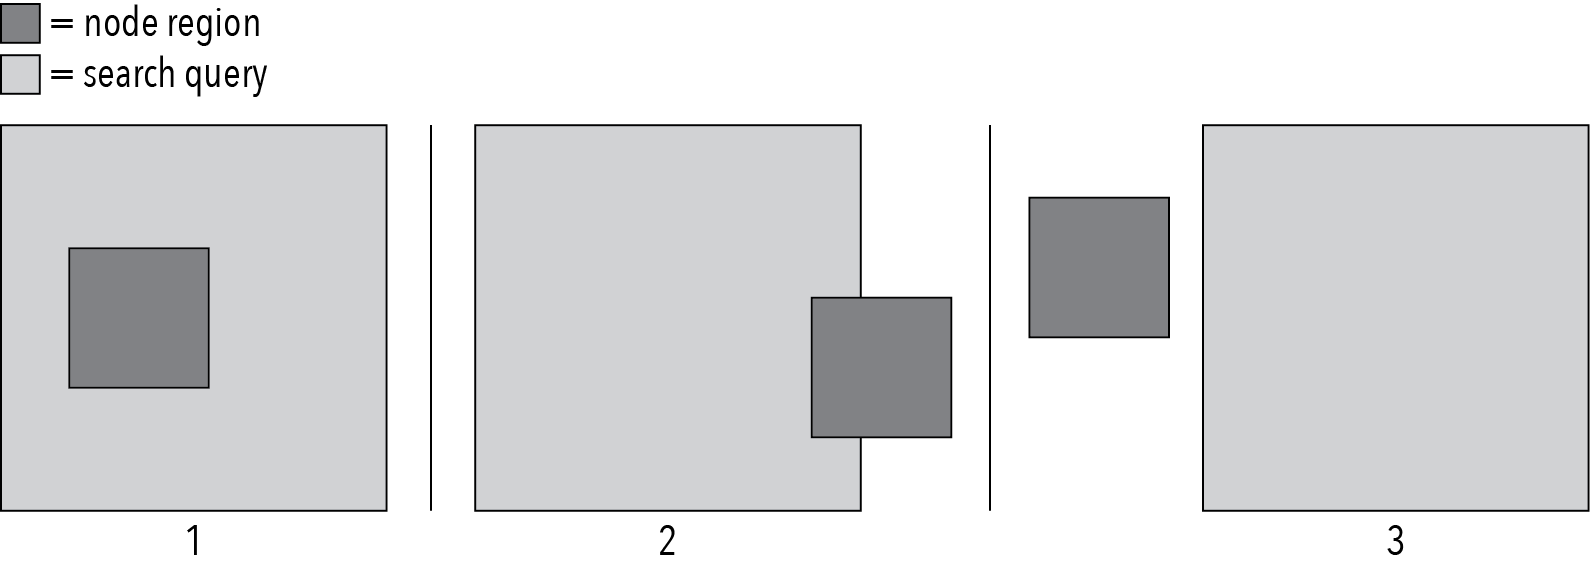
\includegraphics[width = 1.0\textwidth]{pictures/search_query_overlap.png}
    \caption{\DIFaddFL{The three different situations which can occur between a search query and the region of a node}}\label{fig:kdsearchoverlap}
\end{figure}

\DIFaddend In order to search in this tree, we introduce the term \emph{region}. \DIFdelbegin \DIFdel{A }\DIFdelend \DIFaddbegin \DIFadd{The }\DIFaddend region of a node \DIFdelbegin \DIFdel{is the area of which its point lie within}\DIFdelend \DIFaddbegin \DIFadd{$v$ is the smallest axis-aligned area which contains all the points in the subtree of $v$}\DIFaddend . The root contains all points and has the biggest region. Since each node contains a line dividing its points between both of its children, we can use this line to \DIFdelbegin \DIFdel{narrow the region of }\DIFdelend \DIFaddbegin \DIFadd{decrease the size of the regions of }\DIFaddend both children. Doing this halves the amount of points lying within \DIFdelbegin \DIFdel{the region. Now given a }\DIFdelend \DIFaddbegin \DIFadd{each child region. As shown on figure~\ref{fig:kdsearchoverlap}, given an axis-aligned rectangular }\DIFaddend search query $q = [x_1, x_2] \times [y_1, y_2]$ and a \DIFaddbegin \DIFadd{node in the }\DIFaddend kd-tree one of three things can happen\DIFdelbegin \DIFdel{. }\DIFdelend \DIFaddbegin \DIFadd{:
}\begin{enumerate} 
  \item \DIFaddend The region of \DIFdelbegin \DIFdel{a }\DIFdelend \DIFaddbegin \DIFadd{the }\DIFaddend node can be fully contained in the search query, in which case the entire node and the points contained in its subtree are returned as part of the result. 
  \DIFdelbegin \DIFdel{The region of a }\DIFdelend \DIFaddbegin \item \DIFadd{The search query overlaps, but does not fully contain, the region of the }\DIFaddend node $v$\DIFdelbegin \DIFdel{and the search query can overlap in which }\DIFdelend \DIFaddbegin \DIFadd{. In this }\DIFaddend case the search \DIFdelbegin \DIFdel{continues down the }\DIFdelend \DIFaddbegin \DIFadd{will continue down those }\DIFaddend children of $v$ \DIFdelbegin \DIFdel{if their }\DIFdelend \DIFaddbegin \DIFadd{whos }\DIFaddend region overlaps with the search query.
  \DIFaddbegin \item \DIFaddend Finally the region of \DIFdelbegin \DIFdel{a }\DIFdelend \DIFaddbegin \DIFadd{the }\DIFaddend node and the search query \DIFaddbegin \DIFadd{can }\DIFaddend have nothing in common in which case the search at that node stops. \DIFaddbegin \DIFadd{This check will be done by the parent of the node before recursing into the node. 
}\end{enumerate}

\todo{Indtil nu - skrives der så rigtigt? Er alt konsistent omkring brug af ``this node'' og ``the children of the node'' og region?}

\noindent \DIFaddend If a leaf is visited in the search, the point stored in the leaf is reported as part of the result if it lies within the search query. \DIFaddbegin \DIFadd{Also note that internal nodes of the kd-tree are the root of a smaller kd-tree.
}\DIFaddend 

\DIFdelbegin \DIFdel{Copying a point takes $\mathcal{O}(1)$ time.
Thus, given }\DIFdelend \DIFaddbegin \DIFadd{Given }\DIFaddend a node, the time to report \DIFaddbegin \DIFadd{back }\DIFaddend the points stored in the subtree \DIFdelbegin \DIFdel{at the }\DIFdelend \DIFaddbegin \DIFadd{of that }\DIFaddend node is linear in the number of points reported. \DIFdelbegin \DIFdel{It then }\DIFdelend \DIFaddbegin \DIFadd{Thus, it }\DIFaddend takes $\mathcal{O}(k_v)$ time to report back all the $k_v$ points stored in the subtree of a node $v$ which is fully contained in the search region. \DIFaddbegin \\

\DIFadd{From figure~\ref{fig:kdsearchoverlap} case 1 takes $\mathcal{O}(k_v)$ time and case 3 takes constant time. }\DIFaddend In order to \DIFdelbegin \DIFdel{bound the case where the region of a node }\DIFdelend \DIFaddbegin \DIFadd{find the time of a search query to the kd-tree, we need to obtain a bound on the time of case 2. We need to obtain a bound on the amount of nodes visited which }\DIFaddend is not fully contained in the search region\DIFdelbegin \DIFdel{, a vertical line }\DIFdelend \DIFaddbegin \DIFadd{. These are the nodes where an edge of the search query passes through their regions. Consider a search query where one of the edges passes }\DIFaddend through the region of the root\DIFdelbegin \DIFdel{will be used. Conceptually, this vertical line can serve as either the left or right edge of the search region. Consider that the search region does not fully contain regions of any node, this linewill describe }\DIFdelend \DIFaddbegin \DIFadd{. This edge can be thought of as infinitely long. Without loss of generality, we pick it to be a horizontal line, as seen on figure~\ref{fig:kd_bound}. }\\

\begin{figure}[h]
    \centering
    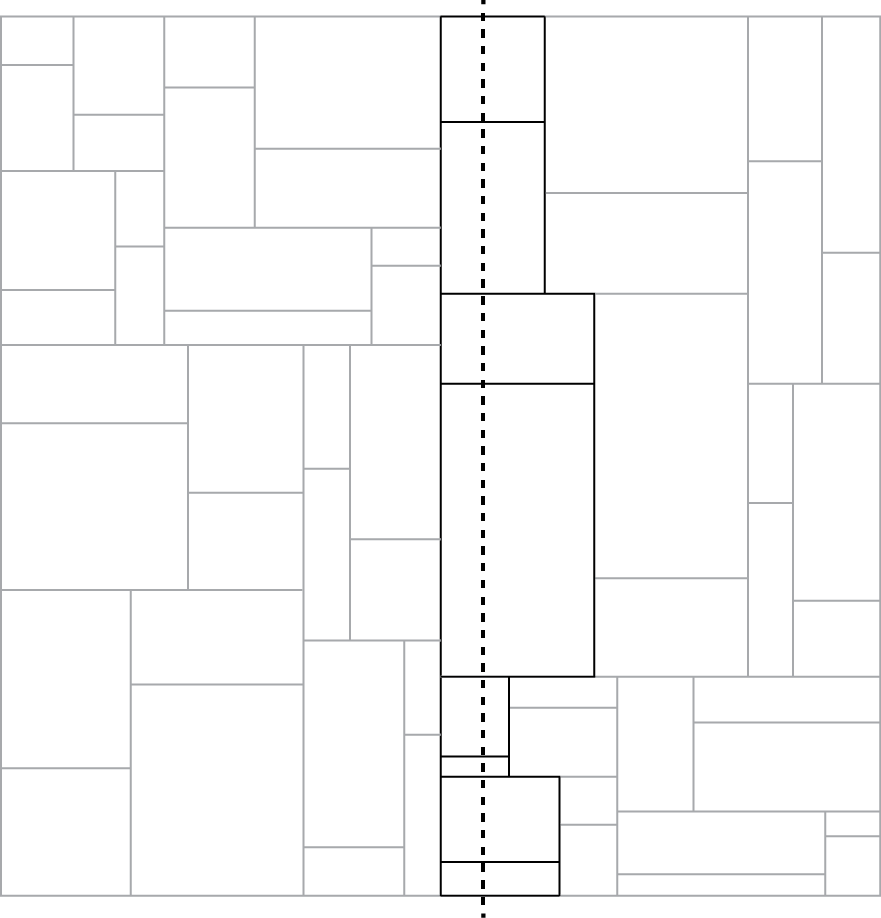
\includegraphics[width = 0.65\textwidth]{pictures/kd_bound2.png}
    \caption{\DIFaddFL{Example of a horizontal edge through the entire region of the root node}}\label{fig:kd_bound}
\end{figure}

\DIFadd{We want to obtain a bound on }\DIFaddend the amount of regions \DIFdelbegin \DIFdel{the search query overlaps}\DIFdelend \DIFaddbegin \DIFadd{this edge can pass through}\DIFaddend . Let $Q(n)$ describe the amount of regions the \DIFdelbegin \DIFdel{vertical }\DIFdelend \DIFaddbegin \DIFadd{horizontal }\DIFaddend line intersects. In order to find the amount of regions intersected by the line, we need to recall how the kd-tree is built. First a region is split in one dimension and then in the other dimension, resulting in four regions every \DIFdelbegin \DIFdel{other step. The vertical }\DIFdelend \DIFaddbegin \DIFadd{two levels of the kd-tree constructed }\todo{Rephrase sentence - argument should be obvious}\DIFadd{. The horizontal }\DIFaddend line will intersect two of these regions. The \DIFdelbegin \DIFdel{vertical }\DIFdelend \DIFaddbegin \DIFadd{horizontal }\DIFaddend line will also intersect the region of the root and one of the two children of the root. The running time of a query to the kd-tree with $n$ points can be described by the recurrence:

\begin{align*}
  Q(n) = \begin{cases}
    \mathcal{O}(1), & \text{if } n = 1,\\
    2 + 2Q(n/4), & \text{if } n > 1
  \end{cases}
\end{align*}

Solving this recurrence gives the solution $Q(n) = \mathcal{O}(\sqrt{n})$. A \DIFdelbegin \DIFdel{vertical }\DIFdelend \DIFaddbegin \DIFadd{horizontal }\DIFaddend line through the region of the root in a kd-tree will intersect $\mathcal{O}(\sqrt{n})$ regions of the kd-tree\DIFdelbegin \DIFdel{.
}\DIFdelend \DIFaddbegin \DIFadd{, thus bounding the amount of regions of nodes a horizontal line can pass through. The exact same argument can be made for a vertical line.
}\DIFaddend 

%% We can also imagine the regions of the kd-tree to form a $m \times m$ grid in the region of the root. Each region in the grid contains one point, and a vertical line through the grid will intersect $m$ regions - one at each row. Since each region in the grid contains a point, we have $m \times m = n$ which gives $m = \sqrt{n}$. Thus, a vertical line through the region of the root will intersect $\sqrt{n}$ regions.

Searching the kd-tree takes $\mathcal{O}(\sqrt{n} + k)$ time to report $k$ points as a result. When the amount of points reported back as result of the search query is low, the query time per point is relatively high. Another thing to notice is that there is no time penalty per point reported. Just searching through the data structure costs $\mathcal{O}(\sqrt{n})$ time, but the time to report back points \DIFdelbegin \DIFdel{are linear to the amount of points }\DIFdelend \DIFaddbegin \DIFadd{is linear in the number of points reported}\DIFaddend .


\DIFdelbegin \DIFdel{The tree with $n$ points can be represented as flat array with $n$ entries. The $\lceil n/2 \rceil$-th element in the array is the root of the tree. }%DIFDELCMD < \todo{uddyb}
%DIFDELCMD < %%%
\DIFdelend %DIF >  The tree with $n$ points can be represented as flat array with $n$ entries. The $\lceil n/2 \rceil$-th element in the array is the root of the tree. \todo{uddyb}

\section{Range trees}
\label{sect:rangetrees}

The range tree is a data structure which supports range queries. The space complexity of this data structure is $\mathcal{O}(n\lg n)$. A normal query in a range tree uses $\mathcal{O}(\lg^2 n + k)$ time to report $k$ points. This time can be optimized to $\mathcal{O}(\lg n + k)$ without changing the space complexity using \emph{fractional cascading}. We will first look at how the data structure is built and how it is used for range reporting. Then we will introduce fractional cascading and see how that will change the query time. With a space complexity of $\mathcal{O}(n \lg n)$ words this data structure is not going to replace the kd-tree. Instead the range tree will serve as a way to introduce some of the ideas behind the SRS and ORS data structures. \DIFaddbegin \\
\DIFaddend 


Consider a balanced binary search tree with $n$ keys for a $1$-dimensional query \DIFaddbegin \DIFadd{on the x-coordinates}\DIFaddend . In order to answer the query $q = [x_1, x_2]$ the following is done: From the root, travel to the \emph{least common ancestor} of $x_1$ and $x_2$. This is the node whose subtree contains both $x_1$ and $x_2$, \DIFdelbegin \DIFdel{but }\DIFdelend \DIFaddbegin \DIFadd{and }\DIFaddend $x_1$ lies in the left subtree, while $x_2$ lies in the right subtree. From the least common ancestor, travel to both $x_1$ and $x_2$. While traveling to $x_1$, the first step is the left child of \DIFaddbegin \DIFadd{the lowest common ancestor }\DIFaddend $x_1$ \DIFaddbegin \DIFadd{and $x_2$}\DIFaddend . From here, everytime a left child is chosen as the next step in the path, the subtree in the right child will only contain points between $x_1$ and $x_2$. This entire subtree is reported back as results. Symmetrically, the same is done with the path to $x_2$. When a right child is chosen as the next step, the subtree in the left child is reported back as results. In a $1$-dimensional search, when a node \DIFdelbegin \DIFdel{has }\DIFdelend \DIFaddbegin \DIFadd{is the root of }\DIFaddend a subtree which only contains points in the search range, the node is said to be \emph{fully contained}.

A balanced binary search tree has a space complexity of $\mathcal{O}(n)$. Reporting back the points stored in a subtree requires time linear to the amount of points in the subtree. Travelling from the root to $x_1$ and $x_2$ requires $\mathcal{O}(\lg n)$ time. Hence, the query time of a $1$-dimensional search query is $\mathcal{O}(\lg n + k)$.

Range reporting in a $2$-dimensional space on the kd-tree is done by using $1$-dimensional sub-queries. The kd-tree alternates in which dimension the search is performed. The range tree also searches by using $1$-dimensional sub-queries, but instead of alternating between dimensions, it separates them. Given a search query $q = [x_1, x_2] \times [y_1, y_2]$, it will first find the points lying in the range of $[x_1, x_2]$. Among those points, it will find the points lying in the range of $[y_1, y_2]$. This leaves us with all the points lying in the search query.

Doing the first $1$-dimensional search is exactly what is accomplished using a balanced binary search tree. A balanced binary search tree is built to support range search on the x-axis of all of the points. We will call this tree the primary tree. Then for each internal node in the primary tree a new balanced binary search tree is built \DIFdelbegin \DIFdel{to support range search on the y-axis of the }\DIFdelend \DIFaddbegin \DIFadd{on all }\DIFaddend points in the \DIFaddbegin \DIFadd{leaves of the }\DIFaddend subtree of that node. We call these balanced binary search trees for auxiliary trees. The primary tree holds pointers to the auxillary tree for each node.

A range query $q = [x_1, x_2] \times [y_1, y_2]$ on the range tree is answered in the following way. From the least common ancestor of $x_1$ and $x_2$, the search travels down to $x_1$ and $x_2$. On the way to $x_1$ and $x_2$, each node that is fully contained in $[x_1, x_2]$ will be flagged. Using the auxilliry tree of each node that is flagged, a search will be done to find the points in the range $[y_1, y_2]$.

The height of a balanced binary search tree containing $n$ points is $\lg n$. Each point $p$ in the primary tree is only stored in the auxillary trees of nodes on the path to the leaf containing the point $p$. This means that each point $p$ is only stored once per level in the primary tree. Each auxillary tree uses space linear to the amount of points it holds. Thus, the space complexity of a range tree is bounded by $\mathcal{O}(n \lg n)$.

The query time for each auxillary tree that is searched is $\mathcal{O}(\lg n + k_v)$, where $k_v$ is the amount of points that is reported back by the auxillary tree at the node $v$ in the primary tree. The amount of auxillary trees which will be searched is bounded by the length of the path from the least common ancestor of $x_1$ and $x_2$ to the leaves containing $x_1$ and $x_2$. This path can at most visit two nodes per level of the primary tree, and the length is thus bounded by $\mathcal{O}(\lg n)$. The query time of a range search in the range tree is then 

\begin{align*}
  \sum\limits_{v} \mathcal{O}(\lg n + k_v) = \mathcal{O}(\lg^2 n + k)
\end{align*}

\noindent where $v$ are the nodes flagged on the path to $x_1$ and $x_2$ from their least common ancestor. \\

Fractional cascasding can be used to speed up the query time without changing the space complexity of the data structure. Instead of using a balanced binary search tree as the auxillary data structure, we are going to use an array. This array will contain the same points as the auxillary balanced binary search tree did. The points in the array will be sorted by their y-coordinate. At the node $v$, each entry in the array \DIFaddbegin \DIFadd{$A_v$}\DIFaddend will contain a point and two pointers. One pointer will be pointing to an entry in the auxillary array of the left child of $v$, while the other pointer will be pointing to an entry in the auxillary array of the rigth child of $v$. We call these the left pointer and the right pointer, respectively. Suppose that $A_v[i]$ stores a point $p$. Then the left pointer \DIFdelbegin \DIFdel{from }\DIFdelend \DIFaddbegin \DIFadd{at }\DIFaddend $A_v[i]$ will be pointing to the first entry in the left childs auxillary array containing a point with a y-coordinate greater or equal to $p_y$. The same applies to the right pointer of $A_v[i]$, pointing to the right child instead of the left child. \\

\DIFaddbegin \begin{figure}[h]
    \centering
    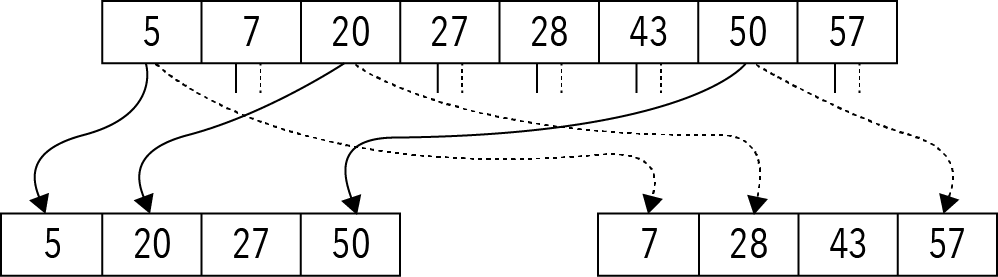
\includegraphics[width = 0.95\textwidth]{pictures/fractional_cascading.png}
    \caption{\DIFaddFL{Example of an fractional cascading}}\label{fig:fractional}
\end{figure}


\DIFaddend Searching the range tree with fractional cascasding starts by finding the least common ancestor of $x_1$ and $x_2$. At this node, a binary search is done in order to find the first entry in the auxillary array which y-coordinate is greater or equal to $y_1$. At any given node, we call the position of this entry $\tau$. We walk from the least common ancestor of $x_1$ and $x_2$ to both $x_1$ and $x_2$, finding all the nodes which are fully contained in $[x_1, x_2]$. Each time a left child is \DIFdelbegin \DIFdel{chosen }\DIFdelend \DIFaddbegin \DIFadd{visited }\DIFaddend on the path to $x_1$ or $x_2$, the left pointer is used to update \DIFdelbegin \DIFdel{the position at $\tau$. When }\DIFdelend \DIFaddbegin \DIFadd{$\tau$. The entry at position $\tau_v$ is the first element in $A_v$ which is greater or equal to $y_1$. Finding the index of this element at }\DIFaddend a \DIFaddbegin \DIFadd{child-node is a constant-time operation using the left pointer. Symmetrically, when a }\DIFaddend right child is \DIFdelbegin \DIFdel{chosen }\DIFdelend \DIFaddbegin \DIFadd{visited }\DIFaddend on the path \DIFaddbegin \DIFadd{to $x_1$ and $x_2$}\DIFaddend , the position of $\tau$ is updated using the right pointer. \DIFaddbegin \DIFadd{This can be seen on figure~\ref{fig:fractional} }\DIFaddend When a fully contained node is found, we look in the auxillary array from the position of $\tau$ and $k_v$ entries forward in order to report $k_v$ points back as result. This is done by incrementing the position of $\tau$ until the point at that entry \DIFdelbegin \DIFdel{no longer is }\DIFdelend \DIFaddbegin \DIFadd{is no longer }\DIFaddend within the range of $[y_1, y_2]$. This takes $\mathcal{O}(1+k_v)$ time. The total query time now becomes
%DIF <  Each time a left child is chosen on the path to $x_1$ or $x_2$, the left pointer is used to update which entry in the auxillary array has the first point with a y-coordinate greater or equal to $y_1$. 

\begin{align*}
  \sum\limits_{v} \mathcal{O}(1 + k_v) = \mathcal{O}(\lg n + k)
\end{align*}

\noindent where $v$ are the nodes flagged on the path to $x_1$ and $x_2$ from their least common ancestor.

\section{Composite-number space} 
\label{sect:composite}
In order to ensure all points have unique x-coordinates and unique y-coordinates, the points are translated into \emph{composite-number space}\DIFaddbegin \DIFadd{\mbox{%DIFAUXCMD
\cite{compgeo}
}%DIFAUXCMD
}\DIFaddend . A composite number of two numbers $x$ and $y$ is denoted by $(x \mid y)$. A total ordering on the composite-number space is defined by using lexicographic order. Given two composite numbers $(x_1 \mid y_1)$ and $(x_2 \mid y_2)$, we define the order as
\begin{align*}
  (x_1 \mid y_1) < (x_2 \mid y_2) \iff x_1 < x_2 \text{ or } (x_1 = x_2 \text{ and } y_1 < y_2)
\end{align*}

\noindent Given a set P of $n$ distinct points from $\mathbb{R}^2$, we translate each point $(x,y) \in P$ into composite-number space by assigning the point new set of coordinates: $(x,y) := ( (x \mid y), (y \mid x) )$. No two points will have the same x-coordinate unless the points are identical. The same holds for the y-coordinate.

\noindent In order to perform a range query $q = [x_1, x_2] \times [y_1, y_2]$ in composite-number space, the query will have to be transformed. This transformed range query will be $\hat{q} = [(x_1 \mid -\infty), (x_2 \mid +\infty)] \times [(y_1 \mid -\infty), (y_2 \mid +\infty)]$. It follows that 
\begin{align*}
  (x,y) \in q \iff ( (x \mid y), (y \mid x) ) \in \hat{q}
\end{align*}


\section{Summary}
\label{sect:relsummary}

The kd-tree is a data structure using $\mathcal{O}(n)$ words of space and supports a range query in $\mathcal{O}(\sqrt{n} + k)$ time. It is built by continually subdividing smaller and smaller regions of the tree until a region only contains one point. A range search query will then match the query region to the region of node to see if there is any overlap or full containment. 
\DIFdelbegin \DIFdel{Because building process alternates between subdividing regions by the x-coordinates and subdividing the regions by the y-coordinates, we cannot state anything other than a region completely below another region contains only points which have smaller y-coordinate than the points in the region above it. The same applies for a region entirely to the left of another region: it only contains points which have a smaller x-coordinate than the points in the region to the right of it. This property forces a range query to look in all the regions which the bordes of range query overlaps. }%DIFDELCMD < \todo{Rephrase - ikke alle, men det højeste level}
%DIFDELCMD < %%%
\DIFdelend 

The range tree is a data structure using $\mathcal{O}(n \lg n)$ words of space and support a range query in $\mathcal{O}(\lg n + k)$ time. It is built by creating a tree with $n$ leaves and dividing the points to the leaves, such that all the leaves to the left of a leaf contain points with a smaller x-coordinate than the point at the leaf. All the internal nodes of the tree contain an auxillary tree which has the same property just with the y-coordinate of the points contained in the subtree. This property allows a search query to quickly locate the subtrees containing only points between $[x_1, x_2]$ and $[y_1, y_2]$.

The $\mathcal{O}(\lg n + k)$ running time of the range tree is faster than the $\mathcal{O}(\sqrt{n} + k)$ running time of the kd-tree. However, the $\mathcal{O}(\sqrt{n})$ part is based on a rather pessimistic idea that a range query will overlap, but not fully include, a lot of regions stretching over the two \DIFdelbegin \DIFdel{extreme }\DIFdelend \DIFaddbegin \DIFadd{extrema }\DIFaddend in one dimension.

\chapter{Primary Work}
\label{ch:primarywork}


This chapter will introduce the Simple Range Search and Original Range Search data structures. The Original Range Search data structure by \citet{chanetal} is a tree-like data structure with \DIFdelbegin \DIFdel{some }\DIFdelend auxillary data structures. It has a space complexity of $\mathcal{O}(n)$ and a supports search queries in $\mathcal{O}(\lg\lg n + (1+k)\cdot\lg^\epsilon n)$ time, where $k$ is the amount of results reported \DIFaddbegin \DIFadd{and $\epsilon$ is an arbitrarily small constant greater than $0$}\DIFaddend .

The Simple Range Search data structure is a simplification of the Original Range Search and therefore they have the same underlying data structure. The Simple Range Search data structure has some different auxillary data structures and fewer of them. The data structure has a space complexity of $\mathcal{O}(n)$ and supports search queries in $\mathcal{O}(\lg n + (1+k)\lg^\epsilon n)$ time. Going forward,\emph{ORS} will be used as shorthand for \emph{Original Range Search} and \emph{SRS} will be used as shorthand for \emph{Simple Range Search}.


The SRS data structure has a time complexity of $\mathcal{O}(\lg n + (1+k)\cdot \lg^\epsilon n)$ which is greather than the time complexity of the ORS data structure with $\mathcal{O}(\lg \lg n + (1+k)\cdot \lg^\epsilon n)$. However, the SRS data structure is far more simple - both in code and the auxilary data structures used. \DIFdelbegin \DIFdel{Because there is much more internal communication between the data structures in the ORS data structure and much more code to be executed, it is safe to assume that the }\DIFdelend \DIFaddbegin \DIFadd{The difference between the }\DIFaddend running time constant \DIFdelbegin \DIFdel{hidden in }\DIFdelend \DIFaddbegin \DIFadd{in $\mathcal{O}(\lg \lg n)$ and $\mathcal{O}(\lg n)$ is far greater than the difference between $\lg \lg n$ and $\lg n$. This makes }\DIFaddend the \DIFdelbegin \DIFdel{$\mathcal{O}(\lg \lg n + (1+k)\lg^\epsilon n)$ time complexity of the ORS data structure far exceeds that of the SRS, making the }\DIFdelend SRS data structure faster than the ORS data structure in \DIFdelbegin \DIFdel{practise.
}%DIFDELCMD < \todo{rephrase}
%DIFDELCMD < %%%
\DIFdelend \DIFaddbegin \DIFadd{practice.
}\DIFaddend 

\vspace{4mm}

Each section will start with a \emph{preliminaries} subsection. This subsection will describe some of the auxiliary data structures used in the section. As in \DIFdelbegin \DIFdel{chapter \ref{ch:relatedwork}}\DIFdelend \DIFaddbegin \DIFadd{Chapter~\ref{ch:relatedwork}, }\DIFaddend the main data structures \DIFdelbegin \DIFdel{mentioned }\DIFdelend in this chapter are output-sensitive \DIFaddbegin \DIFadd{and static}\DIFaddend .

\section{Simple Range Search}
\label{sect:simple}

This section will introduce the primary work of this thesis. It will show how the SRS data structure is built and how range reporting is done using the data structure. The data structure uses $\mathcal{O}(n)$ space and supports search queries in $\mathcal{O}(\lg n + (1+k)\cdot \lg^\epsilon n)$ time. This is the same space complexity as the kd-tree. The query time is different in that $\mathcal{O}(\lg n)$ is smaller than $\mathcal{O}(\sqrt{n})$, but there \DIFdelbegin \DIFdel{now is a penalty }\DIFdelend \DIFaddbegin \DIFadd{is a cost }\DIFaddend of $\mathcal{O}(\lg^\epsilon n)$ per point reported. 

The SRS data structure relies heavily on the \emph{ball-inheritance} data structure. The ball-inheritance structure is a tree with $n$ labelled balls at the root. In $\lg n$ steps it will distribute the balls from the root of the tree to $n$ leaves in the tree. Solving the ball-inheritance problem is to follow a ball from any given node to its leaf. \DIFdelbegin \DIFdel{Solving the ball-inheritance problem can be done in $\mathcal{O}(\lg^\epsilon n)$ time using $\mathcal{O}(n)$ words of space}\DIFdelend \DIFaddbegin \DIFadd{We formally define the problem below }\todo{ref?}\DIFaddend . Succint rank queries are an important part of this chapter, playing a key role in solving the \emph{ball-inheritance problem}.


\subsection{Preliminaries}

\subsubsection{Rank Space Reduction}
Given $n$ points from a universe $U$, the rank of a given point in a sorted list of points is defined as the amount of points which preceed it in the list. Given two points $a,b \in U: a < b$ \emph{iff} $rank(a) < rank(b)$. Expanding this concept to 2 dimensions we have a set $P$ of $n$ points on a $U \times U$ grid. We compute \DIFdelbegin \DIFdel{for }\DIFdelend the \emph{x-rank} $r_x$ for each point in $P$ by finding the rank of the x-coordinate \DIFdelbegin \DIFdel{amongst }\DIFdelend \DIFaddbegin \DIFadd{among }\DIFaddend all the x-coordinates in $P$. The \emph{y-rank} $r_y$ finds the rank of y-coordinate \DIFdelbegin \DIFdel{amongst }\DIFdelend \DIFaddbegin \DIFadd{among }\DIFaddend all of the y-coordinates in $P$. Using \emph{rank space reduction} on $P$, a new set $P^*$ is constructed where $(x,y) \in P$ is replaced by $(r_x(x), r_y(y)) \in P^*$. Given a range query $q = [x_1, x_2] \times [y_1, y_2]$, a point $(x,y) \in P$ is found within $q$ \emph{iff} $(r_x(x), r_y(y))$ is found within $q^* = [r_x(x_1), r_x(x_2)] \times [r_y(y_1), r_y(y_2)]$. Computing the set $P^*$ from $P$ using rank space reduction, $P^*$ is said to be in rank space. While the $n$ points could be represented by $\lg U$ bits in $P$, they can now be represented by $\lg n$ bits in $P^*$ with $\lg n \ll \lg U$ when $n \ll U$ which saves memory. Given $n$ points from $U$ we can translate them to rank space by inserting them in an array $A[1..n]$ and sort $A$. A point's index in $A$ is now its rank. In order to translate a search query $q = [x_1, x_2]$ to rank space, we will look up the successor of $x_1$ in $A$ and the predecessor of $x_2$ in $A$. The \DIFdelbegin \DIFdel{indeces }\DIFdelend \DIFaddbegin \DIFadd{indices }\DIFaddend of these two points delimits the search query in rank space. The array $A$ acts as a mapping to and from rank space. \todo{rephrase} When a rank space reduction has been applied and there exists an array $A[1..n]$ mapping the elements to and from rank space, the algorithms used will only use RAM operations on integers of $\mathcal{O}(\lg n)$ bits.

\subsubsection{Predecessor search using binary search}
In order to find the rank space successor or rank space predecessor of a point, a binary search is used on a sorted array of points. This data structure uses $\mathcal{O}(n)$ space and have a query time of $\mathcal{O}(\lg n)$. By locating the first key in the array that is greater than or equal to the search query, the index of that key is the \DIFdelbegin \DIFdel{rank space successor}\DIFdelend \DIFaddbegin \emph{\DIFadd{rank space successor}}\DIFaddend . Similarly, by locating the last key that is smaller in the array, the index of that key is the \DIFdelbegin \DIFdel{ranks space predecessor}\DIFdelend \DIFaddbegin \emph{\DIFadd{rank space predecessor}}\DIFaddend .



\subsubsection{Succint rank queries}
\DIFaddbegin \label{sssect:succintrank}
\DIFaddend Consider an array $A[1..n]$ with elements from some alphabet $\Sigma$. Given an index $i$ in the array, we can \DIFdelbegin \DIFdel{find out }\DIFdelend \DIFaddbegin \DIFadd{report }\DIFaddend how many elements in $A[1..i]$ are equal to $A[i]$. This is called a \emph{rank query}. We want to be able to \DIFdelbegin \DIFdel{answer the }\DIFdelend \DIFaddbegin \DIFadd{compute a }\DIFaddend rank query in constant time using a data structure of $\mathcal{O}(n \lg \Sigma)$ bits. In order to do this, checkpoints are created. For each character in the alphabet $\Sigma$, the checkpoint contains the number of times that character appears in $A[1..i]$, where $i$ is the checkpoint location. Such a checkpoint takes up $\mathcal{O}(\Sigma \lg n)$ bits of space. By placing \DIFdelbegin \DIFdel{each checkpoint }\DIFdelend \DIFaddbegin \DIFadd{the checkpoints }\DIFaddend $\Sigma \lg n$ entries apart of each other, all of the checkpoints use $\mathcal{O}(\frac{n}{\Sigma \lg n} \cdot \Sigma \lg n) = \mathcal{O}(n)$ bits of space.

\DIFdelbegin \DIFdel{Furthermore, for each entry in the array $A$, a smaller sum will be stored. }\DIFdelend Each entry in $A$ contains a character from the alphabet $\Sigma$. At $A[i]$ we \DIFaddbegin \DIFadd{also }\DIFaddend store the amount of times the character at $A[i]$ \DIFdelbegin \DIFdel{appears }\DIFdelend \DIFaddbegin \DIFadd{occurs }\DIFaddend since the last checkpoint. This is a smaller number and can be stored using $\mathcal{O}(\lg (\Sigma \lg n))$ bits per entry in $A$. This is because we only need $\lg x$ bits to store a number which has a maximum value of $x-1$. \DIFdelbegin \DIFdel{Since there is only $\Sigma \lg n$ entries between each checkpoint, this adds up. }\DIFdelend This approach fits the required space bound if $\Sigma \geq \sqrt{\lg n}$ \todo{replace $\sqrt{\lg n}$ with $\lg^\epsilon n$}, because there $\Sigma$ will dominate the complexity. \DIFaddbegin \DIFadd{Hence, storing $n$ entries uses $\mathcal{O}(n\cdot\lg(\Sigma \lg n)) = \mathcal{O}(n\cdot\lg\Sigma) =  \mathcal{O}(n)$ bits }\todo{Inkluderer ``per level''?}\DIFadd{.}\todo{Er det ved ``to dominate'' betyder i dette tilfælde?} \DIFaddend Working under the word-RAM model of computation, we are able to pack the integers into words of $\lg m$ bits, where $m$ is the maximum number which needs to be stored.

For smaller alphabets, another scheme is used. \DIFdelbegin \DIFdel{Checkpoinst }\DIFdelend \DIFaddbegin \DIFadd{Checkpoints }\DIFaddend are still stored at every $\Sigma \lg n$ positions. \DIFaddbegin \DIFadd{These are now called major checkpoints. }\DIFaddend In addition to this, minor checkpoints are added. These minor checkpoints are added at every $\lg \lg n$ positions and contain the amount of times each character is seen since the last major checkpoint. These minor checkpoints take up $\mathcal{O}(\Sigma \lg \lg n)$ bits each. \DIFaddbegin \DIFadd{$A[i]$ now stores the character from the alphabet $\Sigma$ and how many times that character occurs since the last minor checkpoint. }\DIFaddend In order to answer the rank query, a query to the last major checkpoint and the last minor checkpoint has to be made. Given that $\Sigma \lg \lg n \leq \sqrt{\lg n} \cdot \lg \lg n$, the array entries holding the amount of times $A[i]$ is seen since the last minor checkpoint fits into $\mathcal{O}(\sqrt{\lg n} \cdot \lg^2 \lg n)$ bits. Therefore it is possible to store these array entries in plain form, and with the help of a precomputed table of $n^{\mathcal{O}(1)}$ space we can answer rank queries between minor checkpoints in constant time. \todo{Plain form?} \todo{rephrase} \todo{Maybe only need large alphabet +  bit vector. Then can leave out complicated multilevel}

%\noindent \textbf{Ball Inheritance Problem.} Given a perfect binary tree with $n$ leaves, we want to distribute $n$ labelled balls which appear in an ordered list at the root to the leaves in $\lg n$ steps. \todo{Rephrase}. The list of balls at a given node will inherited by its children with each child receiving the same amount of balls. Each level of the tree contains the same amount of balls. Eventually each ball reaches a leaf of the tree and each leaf will contain exactly one ball. The identity of a given ball is a node and the index of the ball in that nodes list. The true identity, the information the ball contains, only lies in the leaf. The \emph{ball-inheritance problem} is to track a ball from a given node to a leaf and report the identity of the leaf. \\


\subsubsection{Ball Inheritance}
\DIFdelbegin \DIFdel{Given }\DIFdelend \DIFaddbegin \DIFadd{Consider }\DIFaddend a perfect binary tree with $n$ leaves and $n$ labelled balls at the root\DIFdelbegin \DIFdel{, the goal is to distribute the balls }\DIFdelend \DIFaddbegin \DIFadd{. The balls have been distributed }\DIFaddend from the root to the leaves \DIFdelbegin \DIFdel{. }\DIFdelend \DIFaddbegin \DIFadd{in $\lg n$ steps, where each node picks one of its children to inherit a given ball. Both children of a node will receive the same amount of balls. }\DIFaddend The balls at the root are contained in an ordered list\DIFdelbegin \DIFdel{and for each ball in a node 's list , one of its children is picked to inherit the ball such that both children recieve the same amount of balls}\DIFdelend \DIFaddbegin \DIFadd{, and they will retain this order at all internal nodes. Each node contains a list of which ball goes to which child}\DIFaddend . The level of a node is defined to be the height of the node from the leaves. The root has the highest level, while each node is one level smaller than its parent. The leaves are at level $0$. Each level of the tree contains the same amount of balls, and at level $i$ each node contains $2^i$ balls. Eventually each ball reaches a leaf of the tree and each leaf will contain exactly one ball. A ball can be identified by a node and the index of the ball in \DIFdelbegin \DIFdel{that node's list}\DIFdelend \DIFaddbegin \DIFadd{the list of that node}\DIFaddend . Given the identity of a ball at any level, it is possible to follow this ball down the tree to \DIFdelbegin \DIFdel{its leaf which contains the actual coordinates of a point}\DIFdelend \DIFaddbegin \DIFadd{a leaf}\DIFaddend . The goal is to track a balls inheritance from a given node to a leaf and report the identity of the leaf. We call the identity of the leaf \DIFdelbegin \DIFdel{, where the actual coordinates reside, the }\DIFdelend \DIFaddbegin \DIFadd{the }\DIFaddend \emph{true identity} of a ball. \DIFdelbegin \DIFdel{When refering to ball inheritance, the words }\emph{\DIFdel{ball}} %DIFAUXCMD
\DIFdel{or }\emph{\DIFdel{point}} %DIFAUXCMD
\DIFdel{can be used interchangebly.}%DIFDELCMD < \todo{Formatering} \\
%DIFDELCMD < %%%
\DIFdelend \DIFaddbegin \todo{Omskriv afsnit til at reflektere at boldene allerede er fordelt}
\DIFaddend 


\subsection{Solving the ball-inheritance problem} 
\label{ssection:solving-ball}

Consider a perfect binary tree with $n$ leaves. At \DIFdelbegin \DIFdel{each level }\DIFdelend \DIFaddbegin \DIFadd{level $m$, each node contains }\DIFaddend a bit vector \DIFdelbegin \DIFdel{$A[1..n]$ is }\DIFdelend \DIFaddbegin \DIFadd{$A_v[1..2^m]$ }\DIFaddend used to indicate which \DIFdelbegin \DIFdel{of a node's children a }\DIFdelend \DIFaddbegin \DIFadd{child-node a }\DIFaddend ball is inherited by: If \DIFdelbegin \DIFdel{$A[i]$ }\DIFdelend \DIFaddbegin \DIFadd{$A_v[i]$ }\DIFaddend is $0$ it means that the ball \DIFdelbegin \DIFdel{with identity }\DIFdelend \DIFaddbegin \DIFadd{at index }\DIFaddend $i$ in that node was inherited by \DIFdelbegin \DIFdel{its }\DIFdelend \DIFaddbegin \DIFadd{the }\DIFaddend left child and $1$ means that it was inherited by \DIFdelbegin \DIFdel{its }\DIFdelend \DIFaddbegin \DIFadd{the }\DIFaddend right child. \DIFaddbegin \DIFadd{The identity of a ball is a node and an index into the list of that node. }\DIFaddend Given a node $v$ and an identity of a ball, we can now calculate the ball's identity in the child node which inherits the ball. The node can answer the query \DIFdelbegin \DIFdel{$rank_v(k) = \Sigma_{i \leq k} A[i]$}\DIFdelend \DIFaddbegin \DIFadd{$rank_v(k) = \Sigma_{i \leq k} A_v[i]$}\DIFaddend . If a ball is inherited by the right child node its new identity at that node is $rank_v(i)$ because that is how many $1$'s that preceed it in the current node. If a ball is inherited by the left child node the new identity is then $i-rank_v(i)$. With this information it is possible to traverse down the tree following a ball from any given node to a leaf. There are $n$ balls per level \DIFdelbegin \DIFdel{which is represented by a bit vector of size $n$ bits per level. Even though conceptually this bit vector is divided out amongst the nodes of that level, we can interchangebly think of it as a bit vector per level or a bit vector per node}\DIFdelend \DIFaddbegin \DIFadd{stored in the bit vectors of the nodes on that level}\DIFaddend . Each level in the tree uses $\mathcal{O}(n)$ bits to store the bit vectors. This adds up to $\mathcal{O}(n \lg n)$ bits, or $\mathcal{O}(n)$ words in all. This trivial solution to the ball-inheritance problem uses $\mathcal{O}(\lg n)$ query time, given that it follows a ball $\mathcal{O}(\lg n)$ steps down to its leaf. The rank function is a constant time query \DIFdelbegin \DIFdel{.}%DIFDELCMD < \todo{henvis til prelim}%%%
\DIFdel{. }%DIFDELCMD < \\
%DIFDELCMD < %%%
\DIFdelend \DIFaddbegin \DIFadd{~\ref{sssect:succintrank}. }\todo{Hvordan skal jeg referere til dette?}
\DIFaddend 


A bit vector is an array with entries from the alphabet $\Sigma = \{0,1\}$, where each entry is used to indicate whether a left or right child has been chosen to inherit a given ball. By expanding the alphabet we can point to the children's children, $\Sigma = \{0,1,2,3\}$, the children's children's children, $\Sigma = \{0,1,2,3,4,5,6,7\}$, and so forth. Expanding the alphabet will use $\mathcal{O}(n \lg \Sigma)$ bits per level. Storing a pointer from level $i$ to level $i+\Delta$ increases the storage space by $\Delta$ bits per ball, but also enables the ball to be inherited by $2^\Delta$ descendants. By expanding the alphabet the query time can be lowered since it is possible to take bigger steps down the tree. \DIFaddbegin \DIFadd{Just like with a parent-to-child step, bigger steps are supported by succint rank queries. In order to determine the identity of a ball $b$ $\Sigma$ levels below, we need to know the destation node and how many balls before $b$ chose the same destation node. Using succint rank queries to determine the rank of a ball $\Sigma$ levels down is thus a constant time query.
}\DIFaddend 

Using this concept, we pick $B$ such that $2 \leq B \leq m$, where \DIFdelbegin \DIFdel{$m$ }\DIFdelend \DIFaddbegin \DIFadd{$m = \lg n$ }\DIFaddend is the height of the tree. All levels that are a multiple of $B^i$ expand their alphabet such that the balls \DIFaddbegin \DIFadd{can also }\DIFaddend reach $B^i$ levels down. If a target level does not exist, the ball points to its leaf. We need at most visit $B$ levels that are multiple of $B^i$ before reaching a level that is multiple of $B^{i+1}$, making it possible to jump down the tree with bigger and bigger steps.

% $\Sigma^{\lg_B \lg n}_i \frac{\lg n}{B^i} \cdot \mathcal{O}(B^i) = \mathcal{O}(\lg n \cdot \lg_B \lg n)$ 
Storing the expanded alphabets at each level that is \DIFaddbegin \DIFadd{a }\DIFaddend multiple of $B^i$ costs $B^i$ bits per ball. The total cost is then 
\begin{align*}
  \sum\limits_{i=1}^{\lg_B \lg n} \frac{\lg n}{B^i} \cdot \mathcal{O}(B^i) = \mathcal{O}(\lg n \cdot \lg_B \lg n)
\end{align*}


\noindent bits per ball, at all levels. With $n$ balls, this is $\mathcal{O}(n \lg_B \lg n)$ words of space with query time of $\mathcal{O}(B \lg_B \lg n)$. If we pick a $B \leq \lg^\epsilon n$ we can reduce $\lg_B \lg n$ to $\lg_{\lg^\epsilon n} \lg n = \frac{1}{\epsilon}$. Thus, the space complexity for the ball-inheritance data structure is $\mathcal{O}(\frac{1}{\epsilon} \cdot n) = \mathcal{O}(n)$ words of space. By picking $B = \lg^{\epsilon / 2} n \geq \lg \lg n$ we can \DIFdelbegin \DIFdel{make the following reduction }%DIFDELCMD < \todo{rigtige ord?} %%%
\DIFdelend \DIFaddbegin \DIFadd{find the upper bound }\DIFaddend on  the query time \DIFaddbegin \DIFadd{as follows}\DIFaddend :
\begin{align*}
  \mathcal{O}(B \lg_B \lg n) &= \mathcal{O}(B \lg \lg n) = \mathcal{O}(\lg^{\epsilon /2} n \cdot \lg \lg n)\\
  &= \mathcal{O}(\lg^{\epsilon / 2} n \cdot \lg^{\epsilon / 2} n) = \mathcal{O}(\lg^\epsilon n)
\end{align*}

\noindent The ball-inheritance problem can \DIFaddbegin \DIFadd{thus }\DIFaddend be solved in $\mathcal{O}(\lg^\epsilon n)$ \DIFaddbegin \DIFadd{time }\DIFaddend using $\mathcal{O}(n)$ words of space.
\todo{Det er fordi $\lg_B \lg n$ er det største $i$ som beskriver $B^i \leq \lg n$ }

\subsection{Solving range reporting}

Consider a perfect binary tree with $n$ leaves. The root contains $n$ points in $2$-d rank space. \DIFdelbegin \DIFdel{Recall that when distributing points in a binary tree, }\DIFdelend \DIFaddbegin \DIFadd{The elements in }\DIFaddend the \DIFaddbegin \DIFadd{ball-inheritance structure are points, so the }\DIFaddend words \emph{ball} and \emph{point} can be used interchangeably. \DIFdelbegin \DIFdel{These }\DIFdelend \DIFaddbegin \DIFadd{The }\DIFaddend $n$ balls at the root of the tree are sorted by their y-rank. When distributing the balls for inheritance, a node will give both its children half of its balls: the lower half sorted by the x-rank to its left child and the upper half by x-rank to its right child. The order of the balls in a child node will be the same as the parent node. The actual coordinates of the balls are only stored at the leaves. This is how the ball-inheritance data structure was described in the previous section. The ball distribution has been specified. With this distribution, some facts about the tree can be stated. We know that the x-coordinates of the balls in the leaves are sorted from left to right - smallest to highest. The way the balls are distributed from the root, the x-coordinates are responsible for the inheritance path. \todo{rephrase} Because the nodes are sorted by their y-rank in the root node and that they keep this order, the balls in a node list at any given node is ordered by their y-rank. These two facts will be used to solve the range reporting.

\DIFaddbegin \noindent \DIFaddend Since the actual coordinates of the points are only stored once, this data structure uses linear space. \\

Given a range query $q = [x_1, x_2] \times [y_1, y_2]$ the rank successors of $x_1$ and $y_1$ and the rank predecessors of $x_2$ and $y_2$ are looked up. We know from section \todo{ref} that a range query can be translated to a rank space query. We call these $\hat{x}_1, \hat{y}_1, \hat{x}_2$ and $\hat{y}_2$. We now have our query $q$ in rank space: $\hat{q} = [\hat{x_1}, \hat{x_2}] \times [\hat{y_1}, \hat{y_2}]$. We use $\hat{x}_1$ and $\hat{x}_2$ to find the lowest common ancestor, $LCA(\hat{x}_1, \hat{x}_2)$. This node's subtree contains at least all the points with an x-coordinate between $x_1$ and $x_2$. \\

At the root we mark the positions of $\hat{y}_1$ and $\hat{y}_2$ on the bit vector. This range indicates which balls lie within the range of $[y_1, y_2]$. \DIFdelbegin \DIFdel{Going forward we will use }\DIFdelend $i_v$ and $j_v$ \DIFdelbegin \DIFdel{to indicate }\DIFdelend \DIFaddbegin \DIFadd{will denote }\DIFaddend this range in the bit vector of the node $v$. When searching for points lying within this range, a node will update this range to fit its children. The \DIFdelbegin \DIFdel{new }\DIFdelend updated range at the left child $l$ will be $i_l = i_v - rank_v(i_v)$ and $j_l = j_v - rank_v(j_v)$. The \DIFdelbegin \DIFdel{new }\DIFdelend updated range at the right child $r$ will be $i_r = rank_v(i_v)$ and $j_r = rank_v(j_v)$. This is the same way the rank query was used in section \ref{ssection:solving-ball}. Now instead of just following a given ball, we keep track of a range of balls. \DIFaddbegin \DIFadd{This concept is seen on figure~\ref{fig:bitvectorsplit} }\DIFaddend \\

Traversing from the root to the $LCA$, this y-range will be updated accordingly. We know the positions of the leaves containing $\hat{x}_1$ and $\hat{x}_2$ so we can traverse from the $LCA$ down to each of them. Traversing to $\hat{x}_1$, the first stop is the left child of the $LCA$. From here, each time a node selects its left child as the path to $\hat{x}_1$ we know that the subtree contained in the right child only contains points \DIFaddbegin \DIFadd{with x-coordinates }\DIFaddend between $x_1$ and $x_2$. Symmetrically, the same applies when going right from the $LCA$: Each time a node selects a right child on the path to $\hat{x}_2$ the subtree contained in the left child only contains points between $x_1$ and $x_2$. Such a subtree is said to be fully contained. This concept is seen on figure \ref{fig:LCA}. \\

Each time a fully contained subtree is found, we want to follow all the balls lying in the y-range of the root of the subtree to their leaves. This is exactly what the ball-inheritance solves: We are given a list of ball identities and want to find their actualy coordinates. Finding a ball's coordinate from here takes $\mathcal{O}(\lg^\epsilon n)$ time per ball.

\DIFdelbegin %DIFDELCMD < \begin{figure}[H]
%DIFDELCMD <     %%%
\DIFdelendFL \DIFaddbeginFL \begin{figure}[h]
    \DIFaddendFL \centering
    \DIFdelbeginFL %DIFDELCMD < 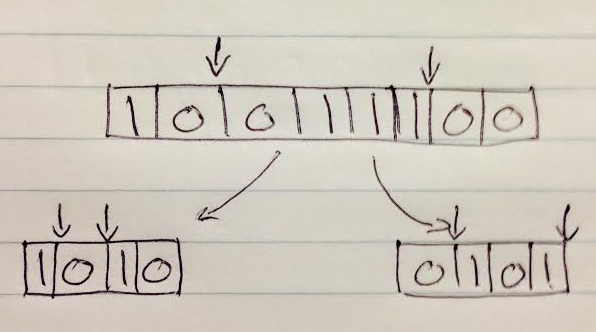
\includegraphics[width=0.6\textwidth]{pictures/bit_vector_split.png}
%DIFDELCMD <     %%%
\DIFdelendFL \DIFaddbeginFL 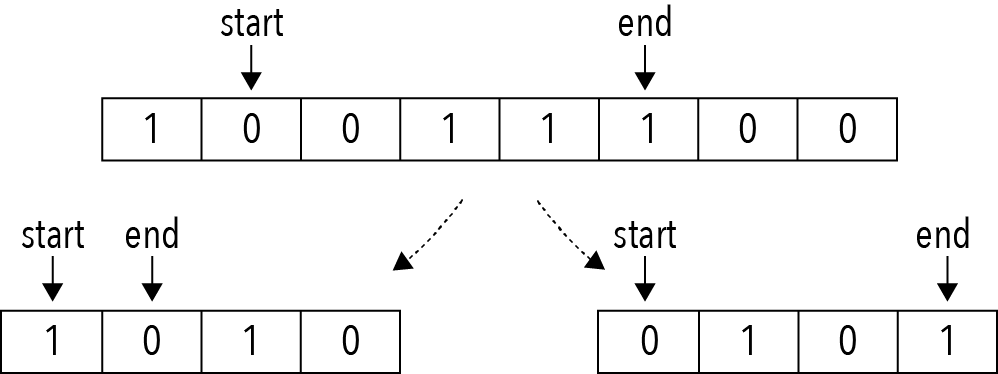
\includegraphics[width=0.95\textwidth]{pictures/bit_vector_split2.png}
    \DIFaddendFL \caption{\DIFdelbeginFL \DIFdelFL{When }\DIFdelendFL \DIFaddbeginFL \DIFaddFL{Example of }\DIFaddendFL nodes \DIFdelbeginFL \DIFdelFL{inherit }\DIFdelendFL \DIFaddbeginFL \DIFaddFL{inheriting }\DIFaddendFL their bit vector ranges from their parent\DIFdelbeginFL \DIFdelFL{, it can become obvious if the entire subtree is contained within the range of $[y_1, y_2]$ or falls without the range}\DIFdelendFL .}
    \label{fig:bitvectorsplit}
\end{figure}


%The data structure is utilized as follows:
%\begin{enumerate}
%    \item Use a binary seach to find the rank space predecessors and successors of $x_1$, $y_1$, $x_2$ and $y_2$. At this point the algorithm will terminate if either rank space range is empty.
%    \item From $LCA(\hat{x}_1, \hat{x}_2)$, both $\hat{x}_1$ and $\hat{x}_2$ will be visited. The range y-rank range found in step $1$ will be updated from the root to this $LCA$ and updated from the $LCA$ to $\hat{x}_1$, $\hat{x}_2$ and all the subtrees between them.
%    \item Each time a fully included subtree is visited, we determine which balls falls within the y-range and use the ball-inheritance structure to travel to its leaf. When a leaf is visited, its actual coordinates will be reported back as a result.
%\end{enumerate}

The actual coordinates of the points are only stored at the leaves which then takes up $\mathcal{O}(n)$  words of space. The rest of the tree contains $\lg n$ levels of bit vectors of $n$ bits taking $\mathcal{O}(n \lg n)$ bits, $\mathcal{O}(n)$ words. Looking up the rank-space predecessor and successor of $x_1, x_2, y_1$ and $y_2$ using a simple binary search at the root requires $\mathcal{O}(n)$ space and $\mathcal{O}(\lg n)$ time. Summing it up, the entire data structure uses $\mathcal{O}(n)$ words of space. 

Walking from the root to the $LCA$ requires $\mathcal{O}(\lg n)$ steps. Visiting $\hat{x}_1$ and $\hat{x}_2$ requires $\mathcal{O}(\lg n)$ steps each. Visiting each of the $k$ leaves in the subtrees between $\hat{x}_1$ and $\hat{x}_2$ ,containing the points which will be reported as a result, takes $\mathcal{O}(k \cdot \lg^\epsilon n)$ time.

This adds up to $\mathcal{O}(\lg n + (1+k)\cdot\lg^\epsilon n)$ query time to report $k$ points as results. \DIFdelbegin \DIFdel{An empty range can be detected by the binary search at the root. There might not be any points with an x-coordinate in $[x_1, x_2]$ or any points with an y-coordinate in $[y_1, y_2]$. If the binary search does not report an empty range, we proceed with the search. }%DIFDELCMD < \todo{Forklar hvordan $\lg^\epsilon n$ opstår fra ``solving ball-inheritance}
%DIFDELCMD < %%%
\DIFdelend \DIFaddbegin \todo{Tilføj en sætning eller to - just remake this}
\DIFaddend 

\DIFdelbegin %DIFDELCMD < \begin{figure}[H]
%DIFDELCMD <     %%%
\DIFdelendFL \DIFaddbeginFL \begin{figure}[h]
    \DIFaddendFL \centering
    \DIFdelbeginFL %DIFDELCMD < 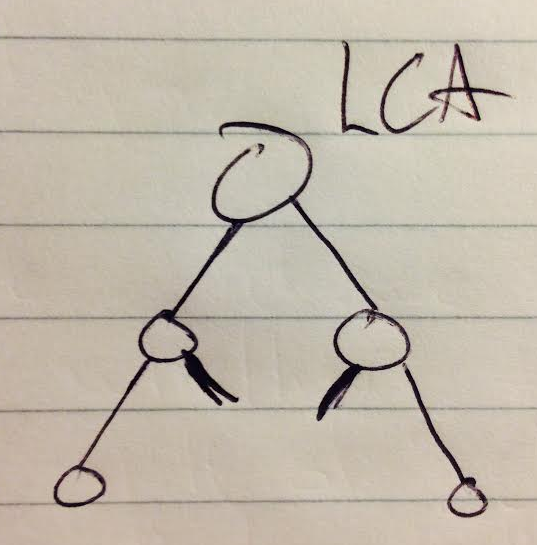
\includegraphics[width=0.6\textwidth]{pictures/LCA.png}
%DIFDELCMD <     %%%
\DIFdelendFL \DIFaddbeginFL 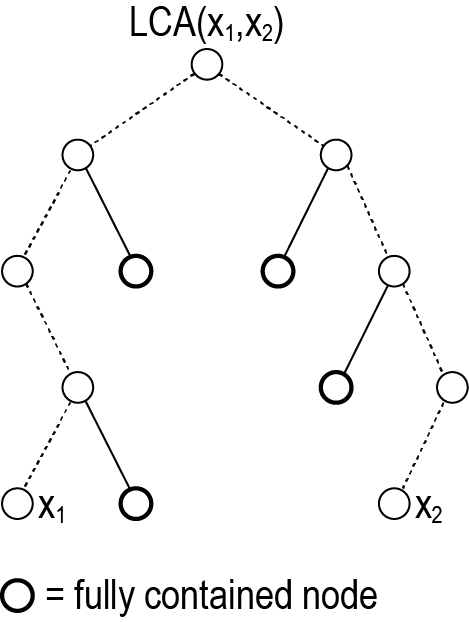
\includegraphics[width=0.6\textwidth]{pictures/LCA2.png}
    \DIFaddendFL \caption{Traversing left from the LCA, each right subtree contains x-coordinates between $x_1$ and $x_2$. Traversing right from the LCA the same holds for left subtrees. \DIFaddbeginFL \DIFaddFL{Dotted line represent the path from the lowest common ancestor of $x_1$ and $x_2$ to $x_1$ and $x_2$}\DIFaddendFL }
    \label{fig:LCA}
\end{figure}


\section{Original Range Search}
\label{sect:original}

This section describes the ORS data structure. While the theoretical work of this thesis is a simplification of this data structure, the ORS can also be viewed as an extension \DIFdelbegin %DIFDELCMD < \todo{Rigtige ord?} %%%
\DIFdelend of the SRS. The ORS data structure will \underline{not} be implemented, but serves as a theoretical background for the SRS. The main property the SRS and ORS share is that the underlying data structure is the ball-inheritance data structure and solving the range reporting heavily relies on solving the ball-inheritance problem.

Utilizing the ball-inheritance structure, \citet{chanetal} propose a \DIFaddbegin \DIFadd{theoretically }\DIFaddend better solution for orthogonal range search queries than the one of the Simple Range Search data structure: 
\begin{customthm}{2.1}\label{theorem21}
for any $2 \leq B \leq \lg^\epsilon n$, we can can solve $2$-d orthogonal range reporting in rank space with $\mathcal{O}(n \lg_B \lg n)$ space and $(1+k)\mathcal{O}(B \lg \lg n)$ query time.
\end{customthm}

In this section some supporting data structures will be introduced. Then we will show how the ball-inheritance is used in conjunction with these data structures to find the points within a search query $q = [x_1, x_2] \times [y_1, y_2]$.

\subsection{Preliminaries}

\subsubsection{Range minimum queries}
In order to find the smallest element in a range, a succint data structure will be used. This data structure can solve the \emph{range minimum query} problem and will be referred to as RMQ. 
Consider an array $A$ with $n$ comparable keys, this succint data structure allows finding the index of the minimum key in the subarray $A[i,j]$. \citet{fischer} introduces a data structure which solves this problem in $2n + \mathcal{O}(n)$ bits of space with constant query time. The construction requires that the array is ordered, which we will see fits into our scheme.

\subsubsection{Rank space \DIFdelbegin \DIFdel{predessecor }\DIFdelend \DIFaddbegin \DIFadd{predecessor }\DIFaddend search}
In order to look up the rank space predecessor of a given coordinate, another succint data structure will be used. This data structure has a \DIFdelbegin \DIFdel{smaller }\DIFdelend \DIFaddbegin \DIFadd{worse }\DIFaddend space complexity than the RMQ \DIFdelbegin \DIFdel{, but has }\DIFdelend \DIFaddbegin \DIFadd{and }\DIFaddend a bigger query time.
Given a sorted array $A[1..n]$ of $\omega$-bit integers, predecessor search queries in $\mathcal{O}(\lg \omega)$ time is supported using $\mathcal{O}(n \lg \omega)$ bits of space with \DIFdelbegin \DIFdel{oracle access }\DIFdelend \DIFaddbegin \emph{\DIFadd{oracle access}} \DIFaddend to the entries in the array. Since $\mathcal{O}(n \lg \omega)$ bits of space is not enough to store $n$ $\omega$-bit integers, the data structure will only store part of each $n$ elements and defer the look-up operation to an \DIFdelbegin \DIFdel{oracle machine}\DIFdelend \DIFaddbegin \emph{\DIFadd{oracle machine}}\DIFaddend . For this purpose a Patricia trie \cite{morehaste} is used to store \DIFdelbegin \DIFdel{the }\DIFdelend some parts of the $n$ $\omega$-bit integers and find which entries in the array $A$ which has to be looked up by the oracle machine. \DIFdelbegin %DIFDELCMD < \todo{Bør jeg uddybe hvordan triet virker? artikel af Ferragina og Grossi snakker om hvordan Patricia træet virker}
%DIFDELCMD < %%%
\DIFdelend \DIFaddbegin \DIFadd{The oracle machine is some data structure that, given an index $i$, can return $A[i]$. Note that $\mathcal{O}(n)$ is less than the bits needed to store $A$. Thus, only the index of the minimum key in $A[i,j]$ can be returned, not the actual key.
}\DIFaddend 

\subsubsection{Finding the lowest common ancestor}
In the Simple Range Search, the lowest common ancestor of $x_1$ and $x_2$ was found by following the path from the root of the tree to both $x_1$ and $x_2$. The last node both paths shared was then the lowest common ancestor. This way of finding the lowest common ancestor takes $\mathcal{O}(\lg n)$ time which is too big for the Original Range Search.
In order to look up the lowest common ancestor of $x_1$ and $x_2$ in constant time, we are going to look at the binary representation of $x_1$ and $x_2$. First we look at $x_1 \oplus x_2$. The number of zero bits from to the start to the first one bit describes the amount of nodes the two paths have in common. We denote this number $b$. This will tell us to look on level $\lg n - b$. The number that the first $b$ bits of $x_1$ describes is the identity of the lowest common ancestor of $x_1$ and $x_2$ on level $\lg n - b$. \DIFaddbegin \DIFadd{Modern machines have an instruction for finding the most significant set bit of a number in constant time. }\DIFaddend Thus, the lowest common ancestor of $x_1$ and $x_2$ can be found in constant time.


\subsection{Solving range reporting}

With a solution to the ball-inheritance problem, \citet{chanetal} propose the following: 
\begin{customlem}{2.4}\label{lemma24}
if the ball inheritance problem can be solved with space $S$ and query time $\tau$, $2$-d range reporting can be solved with space $\mathcal{O}(S+n)$ and query time $\mathcal{O}(\lg \lg n + (1+k) \tau)$.
\end{customlem}


The ball distribution scheme of this data structure is the same as the simplified range search of section \ref{ssection:solving-ball}. Having distributed the $n$ points from the root to the leaves, additional data structures are required in order to answer the range queries. For each node in the tree that is a right child a range minimum query structure is added. The indices are the y-rank and the keys are the x-rank that the given node contains. A range maximum query structure is added to \DIFdelbegin \DIFdel{the }\DIFdelend all the nodes which are left children. Each data structure uses $2n + \mathcal{O}(n)$ bits, making it $\mathcal{O}(n)$ bits per level of the tree and $\mathcal{O}(n \lg n)$ bits in all - i.e. $\mathcal{O}(n)$ words of space. \\

In order to support predecessor (and successor) search for the y-rank in the data structure, the rank space predecessor search data structure is added to the tree. This data structure works on an array of the y-ranks, which is already sorted. The points in rank space of $\mathcal{O}(\lg n)$ bits will use $\mathcal{O}(n \lg \lg n)$ bits per level, with $\omega = \lg n$, and $\mathcal{O}(n \lg n \lg \lg n)$ bits in all, which is $\mathcal{O}(n \lg \lg n)$ words. In order to reduce this to linear space we will only place this predecessor search structure at levels which are multiples of $\lg \lg n$. When using the predecessor search from the lowest common ancestor of $\hat{x}_1$ and $\hat{x}_2$, $LCA(\hat{x}_1, \hat{x}_2)$, we go up to the closest ancestor node which has a predecessor structure in order to perform the search there. Searching takes $\mathcal{O}(\lg \lg n)$ time plus $\mathcal{O}(1)$ queries to the ball-inheritance structure. The ball-inheritance structure is exactly the oracle access that the rank space predessecor search needs: At any given node the balls are sorted by their y-rank and given a the identity (the index) of a ball at that node, it can look up the y-coordinate. \todo{y-coordinate of \ldots} Using the ball-inheritance structure we walk at most $\lg \lg n$ steps down while translating the ranks of $y_1$ and $y_2$ to the right and left child of $LCA(\hat{x}_1, \hat{x}_2)$. 

The reason why this structure is necessary for the y-ranks and not the x-ranks, is because of the way the points have been distributed in the ball-inheritance tree: From left to right, the leaves have x-rank $1,2,..n$ so we can easily locate a given range in \DIFdelbegin \DIFdel{x-dimension}\DIFdelend \DIFaddbegin \DIFadd{the x dimension}\DIFaddend , but in order to keep track of the y-dimensional range we need to follow the balls down the ball-inheritance structure. Adding this structure to each $\lg \lg n$ level saves us from going all the way from the root down to the $LCA$. \\

In order to use this data structure to report points in the range of $q = [x_1, x_2] \times [y_1, y_2]$ we follow these steps:
\begin{enumerate}
  \item We find the rank space successor of $x_1$ \DIFdelbegin \DIFdel{, $\hat{x}_1$, }\DIFdelend and the rank space predecessor of $x_2$\DIFdelbegin \DIFdel{, }\DIFdelend \DIFaddbegin \DIFadd{. We call them $\hat{x}_1$ and }\DIFaddend $\hat{x}_2$. We use these to find the lowest common ancestor of $\hat{x}_1$ and $\hat{x}_2$, $LCA(\hat{x}_1, \hat{x}_2)$. This is the lowest node in the tree whose subtree contains at least all the points between $x_1$ and $x_2$. By knowing $\hat{x}_1$ and $\hat{x}_2$, finding the lowest common ancestor is a constant time operation.   
  \item As in step $1$ where we found the rank space of the x-coordinates, we find the rank space coordinates of the y-coordinates, $\hat{y}_1$ and $\hat{y}_2$, inside the left and right child of $LCA(\hat{x}_1, \hat{x}_2)$. \DIFaddbegin \DIFadd{We are only interested in the rank of $y_1$ and $y_2$ among the points stored in the left and right subtree of $LCA(\hat{x}_1, \hat{x}_2)$. }\DIFaddend This step is precisely what the rank space predecessor structure mentioned above supports.
  \item We now descend into the right child of $LCA(\hat{x}_1, \hat{x}_2)$ and use the range minimum query structure to the find the index $m$ (the y-rank) of the point with the smallest x-rank in the range $[\hat{y}_1, \hat{y}_2]$. The y-rank of a point at a node is exactly the identity of the ball going to the leaf storing the point. Knowing the identity of the ball we can use the ball-inheritance structure to follow the path to the leaf to find the actual x-coordinate of the point. If the x-coordinate is smaller than $x_2$ we return the point as a result and recurse into the ranges of $[\hat{y}_1, m-1]$ and $[m+1, \hat{y}_2]$ in order to find more points. \DIFaddbegin \DIFadd{Otherwise we terminate. }\DIFaddend When this is done we apply the same concept to the left child of $LCA(\hat{y}_1, \hat{x}_2)$ using the range maximum query to find points above $x_1$.
\end{enumerate}

\todo{Insert figure to conceptually show we are working our way out from the inside}

The time complexity of step $3$ depends on the use of the ball-inheritance structure. The time to traverse this structure is dependent on the improvements made in \ref{ssection:solving-ball}. An empty range will result in two queries, one query to each child of $LCA(\hat{x}_1, \hat{x}_2)$. In the worst case the amount of queries to the ball-inheritance structure will be twice the number of results reported plus one. Each time a result is found, a recursion is made to both the left and right subrange of that result. If one of the sides constantly fails to find a result, at most two queries are made for each result found. For the final result found, two ranges are recursed into which reports no results.

Conceptually, $LCA(\hat{x}_1, \hat{x}_2)$ describes a point between $x_1$ and $x_2$. Step $3$ selects points that are in the range of $[y_1, y_2]$ moving outwards from the point of $LCA(\hat{x}_1, \hat{x}_2)$, always picking the point closest to $LCA(\hat{x}_1, \hat{x}_2)$ in its decreasing y-range. \todo{rephrase}

Going back to Lemma $2.4$, we see that the time complexity fits: $\mathcal{O}(\lg \lg n)$ time is used for the predecessor search and $\mathcal{O}((1+k)\tau)$ time is used for walking from the children of the $LCA$ to the leaves solving the ball inheritance problem for the $k$ results.

\section{Summary}
\label{sect:summaryprim}

The SRS and ORS data structures both uses $\mathcal{O}(n)$ words of space. Both relies heavily on the ball-inheritance data structure in order to store and retrieve the actual coordinates of points. Both data structures supports retrieval of points through the ball-inheritance data structure in $\mathcal{O}(\lg^\epsilon n)$ time. The main difference between the SRS data structure and the ORS data structure is the rest of the query time: $\mathcal{O}(\lg n)$ for the SRS and $\mathcal{O}(\lg \lg n)$ for the ORS. The ORS data structure relies on more auxillary data structures of greater complexity than the SRS data structure. Thus, the theoretical running time of a range query to ORS is smaller than a range query to the SRS. In practise, it is safe to assume a range query to the SRS is faster than a range query to the ORS. With much more code to be executed and using more advanced auxillary data structures, the running time constant hidden in $\mathcal{O}(\lg \lg n)$ can be quite large. Also,  the factor between $\lg n$ and $\lg \lg n$ is not that big. Given a very large dataset of \DIFdelbegin \DIFdel{$2^64$ }\DIFdelend \DIFaddbegin \DIFadd{$2^{64}$ }\DIFaddend elements as input, \DIFdelbegin \DIFdel{$\lg 2^64 = 64$ and $\lg \lg 2^64 = 6$}\DIFdelend \DIFaddbegin \DIFadd{$\lg 2^{64} = 64$ and $\lg \lg 2^{64} = 6$, which has a factor $\sim10$ difference}\DIFaddend . \\

\DIFaddbegin \DIFadd{The SRS and ORS data structures supports search queries in a manner similar to the range tree. A balanced binary search tree is used to locate the subtrees which is fully contained in $[x_1, x_2]$. From here the range tree uses balanced binary search trees or fractional cascading to locate which of those points are in $[y_1, y_2]$, while the SRS and ORS data structures uses the ball-inheritance structure to decode the y-ranks to actual points. }\\

\DIFaddend Both the SRS data structure and the kd-tree uses $\mathcal{O}(n)$ words of space. This is an attractive property when working on the RAM. Like all the main data structures mentioned in this thesis, the kd-tree and SRS data structure are output-sensitive. A range query to the kd-tree has a running time of $\mathcal{O}(\sqrt{n}+k)$ and a range query to the SRS data structure has a running time of $\mathcal{O}(\lg n + (1+k)\cdot\lg^\epsilon n)$. When $n$ grows, $\mathcal{O}(\sqrt{n})$ grows at a faster rate than $\mathcal{O}(\lg n)$. For each point reported as a result from a range query to the SRS data structure there is a \DIFdelbegin \DIFdel{penalty }\DIFdelend \DIFaddbegin \DIFadd{cost }\DIFaddend of a factor $\mathcal{O}(lg^\epsilon n)$ while \DIFdelbegin \DIFdel{a }\DIFdelend \DIFaddbegin \DIFadd{each point reported as a result from a }\DIFaddend range query to the kd-tree has a \DIFdelbegin \DIFdel{penalty }\DIFdelend \DIFaddbegin \DIFadd{cost }\DIFaddend of a factor $\mathcal{O}(1)$. \DIFdelbegin %DIFDELCMD < \todo{Er det en penalty factor når det er constant time?}%%%
\DIFdel{. }\DIFdelend The $\mathcal{O}(\sqrt{n})$ running time of the range query to the kd-tree is due to a pessimistic idea that a range query will overlap, but not fully include, a lot of regions in the kd-tree. So dependent on the shape of the range query to the kd-tree, the running time can vary a lot. The $\mathcal{O}(\lg n)$ part of the range query to the SRS data structure is due to the initial binary search and to follow the path from the root of the tree to $x_1$ and $x_2$. Thus, the running time of a range query to the SRS data structure will behave more stable (fluctuate less) than the running time of a range query to the kd-tree. 


\todo{Kan man sige noget en sammenligning af de to worst-cases? At den ene er bedre end den anden og det sætter en bedre upper bound?}

Another aspect of range querying is testing for emptiness. When testing for emptiness, a range query can stop the moment a single result is found since it is a test with the binary outcome of ``yes'' or ``no''. The SRS data structure will be able to determine emptiness of a range query with no ball-inheritance queries. Hence, an emptiness query to the SRS data structure can be checked in $\mathcal{O}(\lg n)$ time. The initial binary search to find the rank space query might indicate that there are no points in $[x_1, x_2]$ or $[y_1, y_2]$. If the initial binary search does not indicate an empty range, the range query will continue normally. The moment a query to the ball-inheritance structure is made, the range is not empty and the emptiness test can report back without doing the actual ball-inheritance query. An emptiness query to the kd-tree can checked in $\mathcal{O}(\sqrt{n})$ time. The same argument as before applies: The query might overlap with a lot of regions which it does not fully contain, and within those regions none of the points are within the range. On the other hand, when a fully contained region is found the emptiness test can report back with a result. Given a range query $[x_1, x_2] \times [y_1, y_2]$, the SRS data structure will have a more stable running time for its emptiness test than the kd-tree. The running time of a query made to the kd-tree will fluctuate a lot depending on the shape of the query.
\DIFaddbegin 

\todo{Ting du skal huske at have med i dette kapitel: Decode y-rank i stedet for at slå op i søgetræ. Range-tree imod ball-inheritance}
\todo{Balls per level vs balls per node - hvordan skal det introduceres (og hvor). Rank af bolde i node (per node)}


\part{\DIFadd{Practical}}

\chapter{\DIFadd{Implementation}}

\section{\DIFadd{Language}}

\DIFadd{In order to implement the $SRS$ data structure and the kd-tree, C++11 was used. C++11 is a recent release of C++. C++11 combines the advantages of a modern programming language with the stability and support of a mature language which have been around for more than three decades. C++11 was chosen for several reason: It does not have garbage collection, it is a high level language with support for low level operation and contains libraries for everything needed in this project. The chrono header gives access to a high resolution clock to meassure time. The vector class of the standard template library is very straight-forward container to work with and the underlying structure is a continuous block of memory making it ideal for cache purposes. The algorithm header gives access to convenience functions for generating and sorting data.
}

\section{\DIFadd{Design choices}}

\DIFadd{The theory describes the ball inheritance data structure as a binary tree with internal node and leaves. Each node then has a ball inheritance list to show which ball was inherited by which child. In practise all the ball inheritance lists per level are merged together to one, resulting in $\lg n$ ball inheritance lists in all. Instead of being an actual entity, a node is just defined as which level it is from, where on that levels list its ball inheritance list starts and how many balls its list holds. Since each ball only uses a single bit per level there would have been a lot of space wasted when nodes only held two or four balls in their ball inheritance lists. By having one list per level we can pick one data type to work without independent of how many balls needs to be stored per node. std::uint32}\_t \todo{hvordan skriver jeg det pænt?} \DIFadd{was chosen in this case. It is an unsigned fixed width integer type of $32$ bits.
}


\DIFadd{Skriv om hvordan det virker med enkelte hop. Vi har en look-up til 16 bits. Vi har en sum for hvert 32 bits. At 0 bare er komplementar af 1 når vi tæller.
}

\chapter{\DIFadd{Analysis}}
\DIFaddend 



\chapter{\todo{\dots}}
\label{ch:main}

%% \todo{example of a citation to primary literature: \citeA{lazypropagation2010},

%%%%%%%%%%%%%%%%%%%%%%%%%%%%%%%%%%%%%%%%%%%%%%%%%%%%%%%%%%%%%%%%%%%%%%%

\chapter{Conclusion}
\label{ch:conclusion}

\todo{\dots}

%%%%%%%%%%%%%%%%%%%%%%%%%%%%%%%%%%%%%%%%%%%%%%%%%%%%%%%%%%%%%%%%%%%%%%%

\addcontentsline{toc}{chapter}{Primary Bibliography}
\bibliographystyle{plainnat} 
\begin{thebibliography}{5}
\providecommand{\natexlab}[1]{#1}
\providecommand{\url}[1]{\texttt{#1}}
\expandafter\ifx\csname urlstyle\endcsname\relax
  \providecommand{\doi}[1]{doi: #1}\else
  \providecommand{\doi}{doi: \begingroup \urlstyle{rm}\Url}\fi

\bibitem[Berg et~al.(2008)Berg, Cheong, Kreveld, and Overmars]{compgeo}
Mark~de Berg, Otfried Cheong, Marc~van Kreveld, and Mark Overmars.
\newblock \emph{Computational Geometry: Algorithms and Applications}.
\newblock Springer-Verlag TELOS, Santa Clara, CA, USA, 3rd ed. edition, 2008.
\newblock ISBN 3540779736, 9783540779735.

\bibitem[Chan et~al.(2011)Chan, Larsen, and P\u{a}tra\c{s}cu]{chanetal}
Timothy~M. Chan, Kasper~Green Larsen, and Mihai P\u{a}tra\c{s}cu.
\newblock Orthogonal range searching on the ram, revisited.
\newblock In \emph{Proceedings of the Twenty-seventh Annual Symposium on
  Computational Geometry}, SoCG '11, pages 1--10, New York, NY, USA, 2011. ACM.
\newblock ISBN 978-1-4503-0682-9.
\newblock \doi{10.1145/1998196.1998198}.
\newblock URL \url{http://doi.acm.org/10.1145/1998196.1998198}.

\bibitem[Fischer(2008)]{fischer}
Johannes Fischer.
\newblock Optimal succinctness for range minimum queries.
\newblock \emph{CoRR}, abs/0812.2775, 2008.
\newblock URL \url{http://arxiv.org/abs/0812.2775}.

\bibitem[Fredman and Willard(1993)]{fredman}
Michael~L. Fredman and Dan~E. Willard.
\newblock Surpassing the information theoretic bound with fusion trees.
\newblock \emph{Journal of Computer and System Sciences}, 47\penalty0
  (3):\penalty0 424 -- 436, 1993.
\newblock ISSN 0022-0000.
\newblock \doi{http://dx.doi.org/10.1016/0022-0000(93)90040-4}.
\newblock URL
  \url{http://www.sciencedirect.com/science/article/pii/0022000093900404}.

\bibitem[Grossi et~al.(2009)Grossi, Orlandi, Raman, and Rao]{morehaste}
Roberto Grossi, Alessio Orlandi, Rajeev Raman, and S.~Srinivasa Rao.
\newblock More haste, less waste: Lowering the redundancy in fully indexable
  dictionaries.
\newblock \emph{CoRR}, abs/0902.2648, 2009.
\newblock URL \url{http://arxiv.org/abs/0902.2648}.

\end{thebibliography}


\end{document}

